\documentclass[main.tex]{subfiles}

\begin{document}
	
	\begingroup
	
	\renewcommand{\cleardoublepage}{}
	
	\renewcommand{\clearpage}{}
	
	\chapter{Grocery Task Overview}
	
	\chapterauthor{Everyone}

\textit{This chapter as well as the chapter about the clean up task could sadly not have been finished in time. In the next days, there will follow some explanations about the different tasks, the robot is doing during these two challenges. It will come together as a continious text that will give a less technical overview about all the whole process. The parts that are already written in these two chapters will probably not make much sense without the rest.}

	\section{Goal}

	The goal which has to be achieved in the grocery storing task is to collect objects from a table and place them in a logical position in a shelf. The HSR has to autonomously navigate the environment, it has to manipulate objects like doors and grocery items like chips, bananas etc. furthermore the HSR has to be able to lift items of the table and place them in the shelf where the final position of the moved object should either be grouped with similar objects (similarity is defined by size, color, shape and class) or open a new group apart from items which are not similar. The HSR has 5 minutes to achieve the given task.
	

	\section{Tasks}

		\begin{figure}	
			\centering
			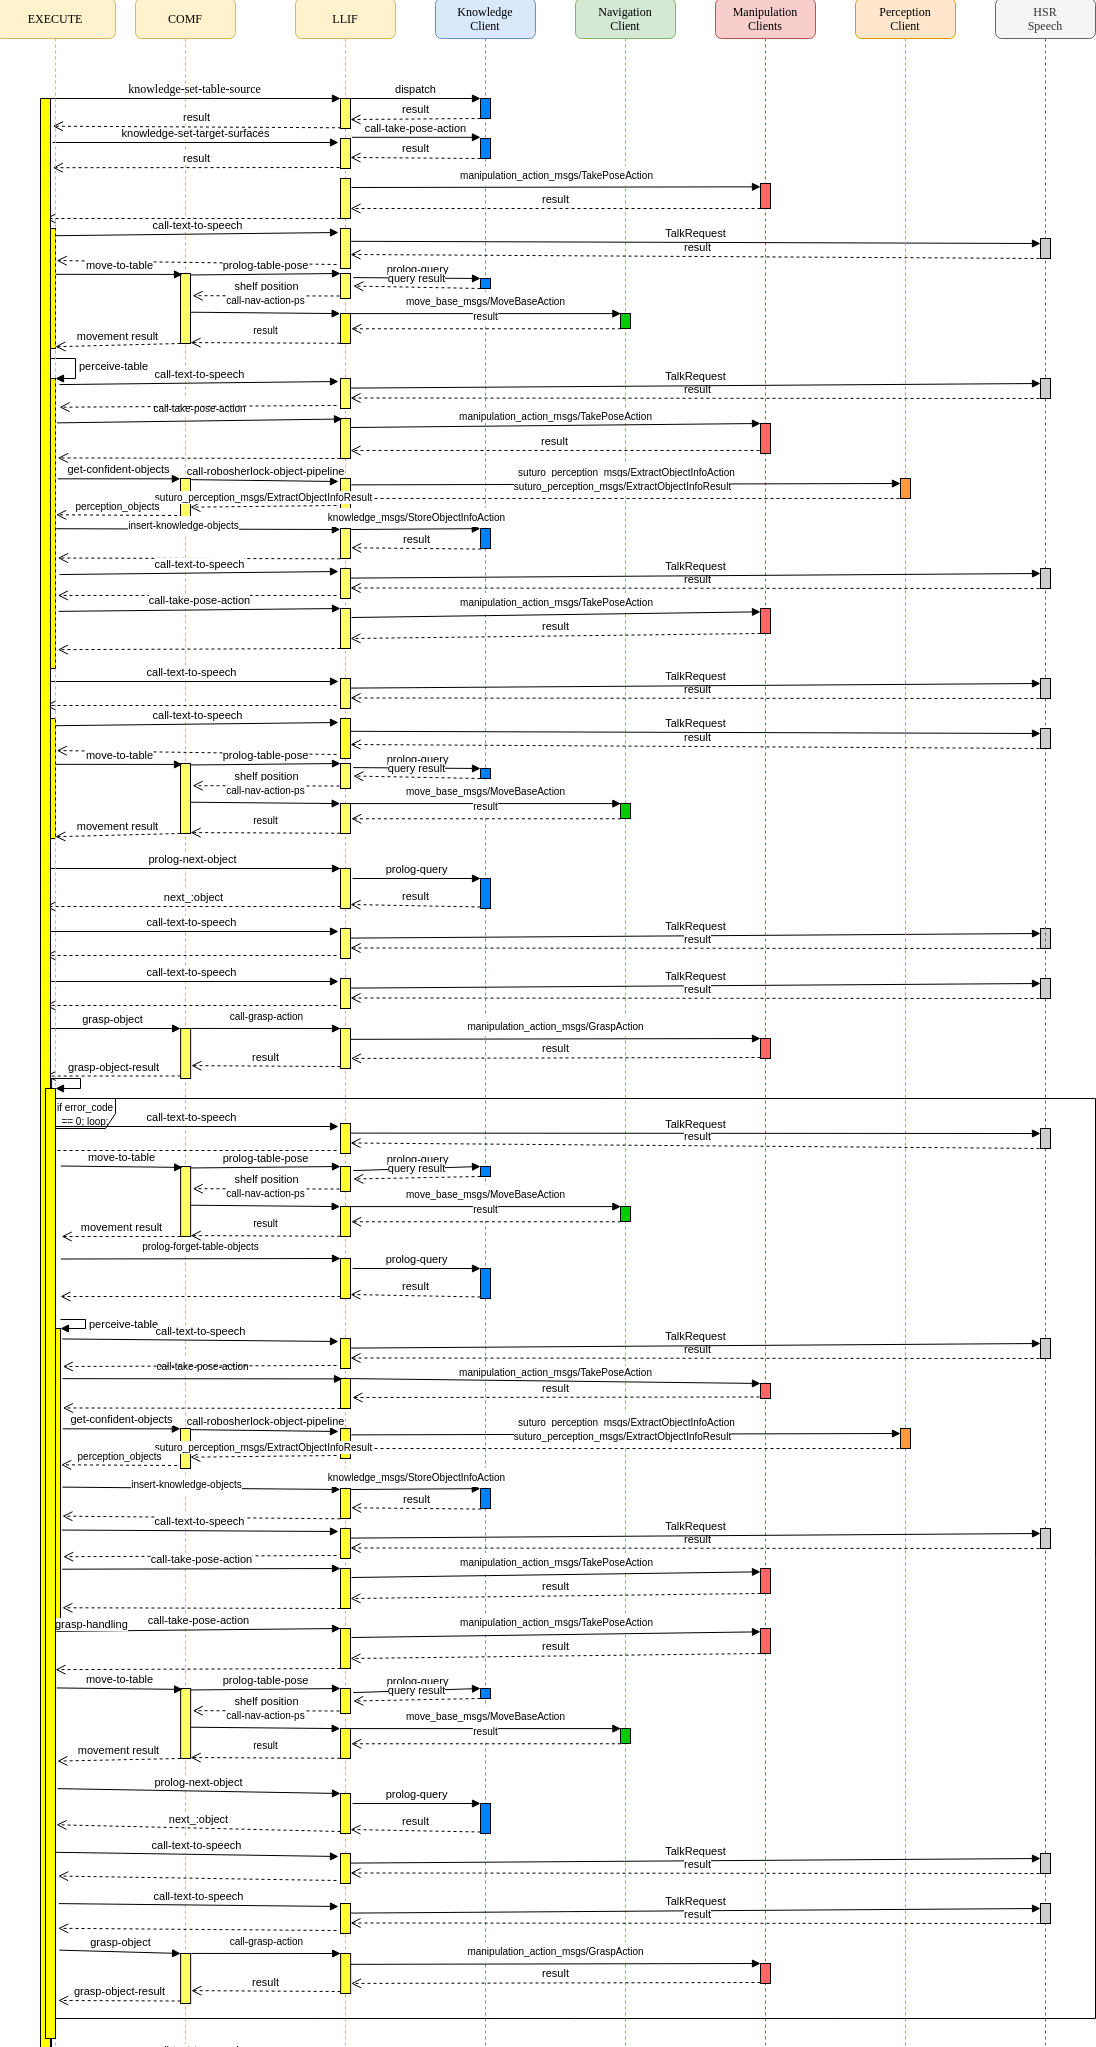
\includegraphics[width=0.85\textwidth]{pictures/diagramms/first-part-grocery-sequence.png}
			\caption{Sequence diagram of the complete run of the grocery storing task \textit{(explanations below)}}
			\label{grocery_seq_01}
		\end{figure}
		\begin{figure}	
			\centering
			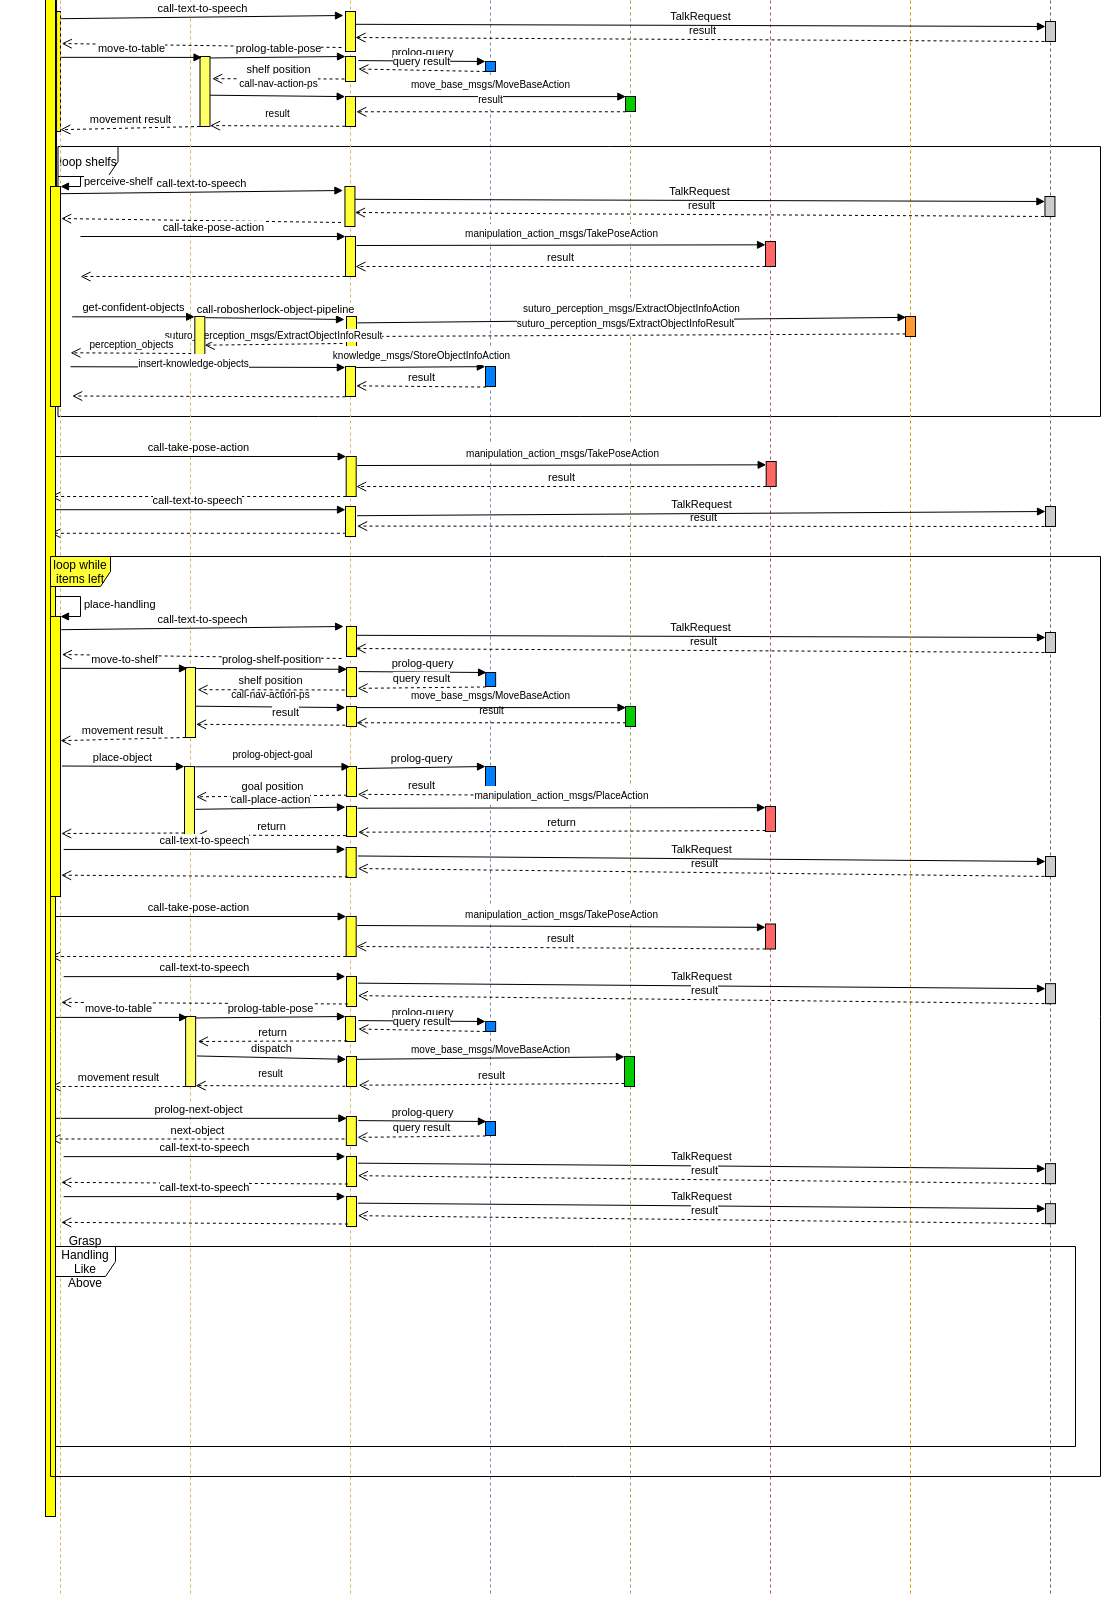
\includegraphics[width=0.85\textwidth]{pictures/diagramms/second-part-grocery-sequence.png}
			\caption{Sequence diagram of the complete run of the grocery storing task \textit{(explanations below)}}
			\label{grocery_seq_02}
		\end{figure}
		\textit{The sequence diagram in figure \ref{grocery_seq_01} and \ref{grocery_seq_01} does not depict when the action servers are running it rather displays the time they are actively used}
	
	\subsection{Setup}
		
	
	In the following subsections the execution and the procedure depicted in figure \ref{grocery_seq_01} and \ref{grocery_seq_02} will be explained in detail and include decisions made which let to this exact plan. Some more detailed challenges will be explained as well.

	% Knowledge: set-tables-source 
	At first the definition of the task is set in knowledge: We want to find objects on all the tables, so all the table surfaces are set as \texttt{source} and we want to place the found objects in shelves, so all the shelves are set as \texttt{target}. This procedure enables Knowledge, to generically work over \texttt{source} and \texttt{target} surfaces regardless of what they actually are.
	
	\subsection{Scan Table}
	
	% Manipulation: take pose action
	The robot is set to the default pose so it doesn't collide with any objects, this could happen if the robot is told to move while in a pose where for example the arm is extended.
	
	% NLP: Talk Request
	
	The talk requests are used to inform the developer as well as the people following the robot or evaluating its behavior about what the robot is about to do. They are also used for safety measures so the robot can warn when it is going to move so bystanders can step aside. 
	
	% Knowledge: get table-poses
	Knowledge finds all the tables available, sorts them by their distance to the robot and then returns the list of their position to Planning, so Planning can determine where to go next.
	
	% Navigation: moveBaseAction
	
	The robot moves to the designated location in this case the table, it will be turned 90° so it is in a pose where perceiving the table isn't hindered by the arm of the HSR. 
	
	% NLP
	Informing that the robot is perceiving the table now.
	
	% Manipuilation: TakePoseAction
	The robot has to take one of 3 perceive poses depending on the heights of the objects he wants to look at.
	
	% Perception: Percieve and return data
	The HSR takes a picture of the scene it is currently looking at and processes it by \textbf{PERCEPTION SCHREIBT HIER BITTE MEHR}
	
	% Knowledge: Store Data
	Knowledge checks the data of the object, that is supposed to be stored. If the class is unknown to knowledge, it is set to other. If the data is valid the object gets added to the knowledge base and the objects at the position of the new object are put into a group.
	% NLP: Talk Request
	
	% Manipulation: Take pose
	Take default pose.
	
	% 2x NLP: Talk
	
	% Knowledge: prolog_ shelf_pose (???)
	
	% Navigation: MoveBaseAction
	Turn the HSR by 90° so he can grasp objects which would not be possible from the pose he took to perceive the objects.
	
	\subsection{Grasp Object}
	
	% Knowledge: next_object
	Ask the KB which is the next object which the robot should deliver to it's target. What the next object should be is determined by \textbf{KNOWLEDGE LEUTE MÜSSEN DAS ERKLÄREN}
	
	% 2x NLP: Talk Request
	
	% Manipulation: GraspAction
	
	% Planning: This whole thing is gonna be looped 
	
	% NLP
	
	% Knowledge: Shelf Positions
Knowledge finds all the shelves available and sorts them, just like the tables before, by their distance to the robot. This way, the Robot can navigate to all the shelves starting with the nearest one to scan the objects already in place.
	
	% Navigation: Move to Shelf
	
	\subsection{Scan shelf floors}
	
	% Planning: Loop through all shelf floors
	
	% NLP
	
	% Manipulation: go into percieve pose
	
	% Perception: Percieve shelf
	
	% Knowledge: Store new Objects
	
	\subsection{Place Object}
	
	% Planning: Loop this while some items are left
	
	% Knowledge: shelf positions
	
	% navigation: move to shelf (???)
	
	% Knowledge: Object goal pose
Knowledge now determines the most suitable position for the Object, it earlier chose to be the next Object. The way this decision is made is discussed later in the Knowledge function documentation (see section \ref{sec:kn_find_surf} under "Finding a goal surface for an Object"). For now it is enough to know, that Knowledge finds not only a suitable surface for that object but also the exact coordinates in the world frame for that object based on its own properties and based all the other known Objects in the scene.
	
	% Manipulation: TakePoseAction
	
	% NLP
	
	% Manipulation: TakePoseAction
	
	% NLP
	
	% Knowledge: table pose
	
	% Knowledge: next_object
	
	% 2x NLP
	
	% Planning: Finish
	
	
	\section{Conclusion}

	We achieved the task blash blash blash ...
	
	
	\endgroup
	
\end{document}
